\subsubsection{Incremento 10}

\myparagraph{Prospetto orario}
In questo incremento, la distribuzione oraria dei componenti del gruppo è la seguente:

{

\rowcolors{2}{azzurro2}{azzurro3}

\centering
\renewcommand{\arraystretch}{1.8}
\begin{longtable}{C{4cm} C{1cm} C{1cm} C{1cm} C{1cm} C{1cm} C{1cm} C{2cm}}

\rowcolor{azzurro1}
\textbf{Nominativo} &
\textbf{RE}&
\textbf{AM}&
\textbf{AN}&
\textbf{PT}&
\textbf{PR}&
\textbf{VE}&
\textbf{Ore totali}\\
\endhead

\MB & 0 & 0 & 0 & 1 & 2 & 1 & 4 \\
\VAS & 0 & 0 & 0 & 2 & 0 & 2 & 4 \\
\FD & 0 & 0 & 0 & 0 & 3 & 3 & 6 \\
\NM & 0 & 0 & 0 & 0 & 4 & 1 & 5 \\
\SB & 1 & 0 & 0 & 0 & 0 & 3 & 4 \\
\GB & 2 & 3 & 0 & 0 & 0 & 0 & 5 \\
\MDI & 0 & 0 & 0 & 1 & 1 & 3 & 5 \\
\textbf{Ore Totali} & 3 & 3 & 0 & 4 & 10 & 13 & 33 \\

\rowcolor{white}
\caption{Distribuzione oraria nell'incremento 10}\\

\end{longtable}
}
\newpage
Il seguente istogramma riassume i dati ottenuti:

\begin{figure}[H]
\centering
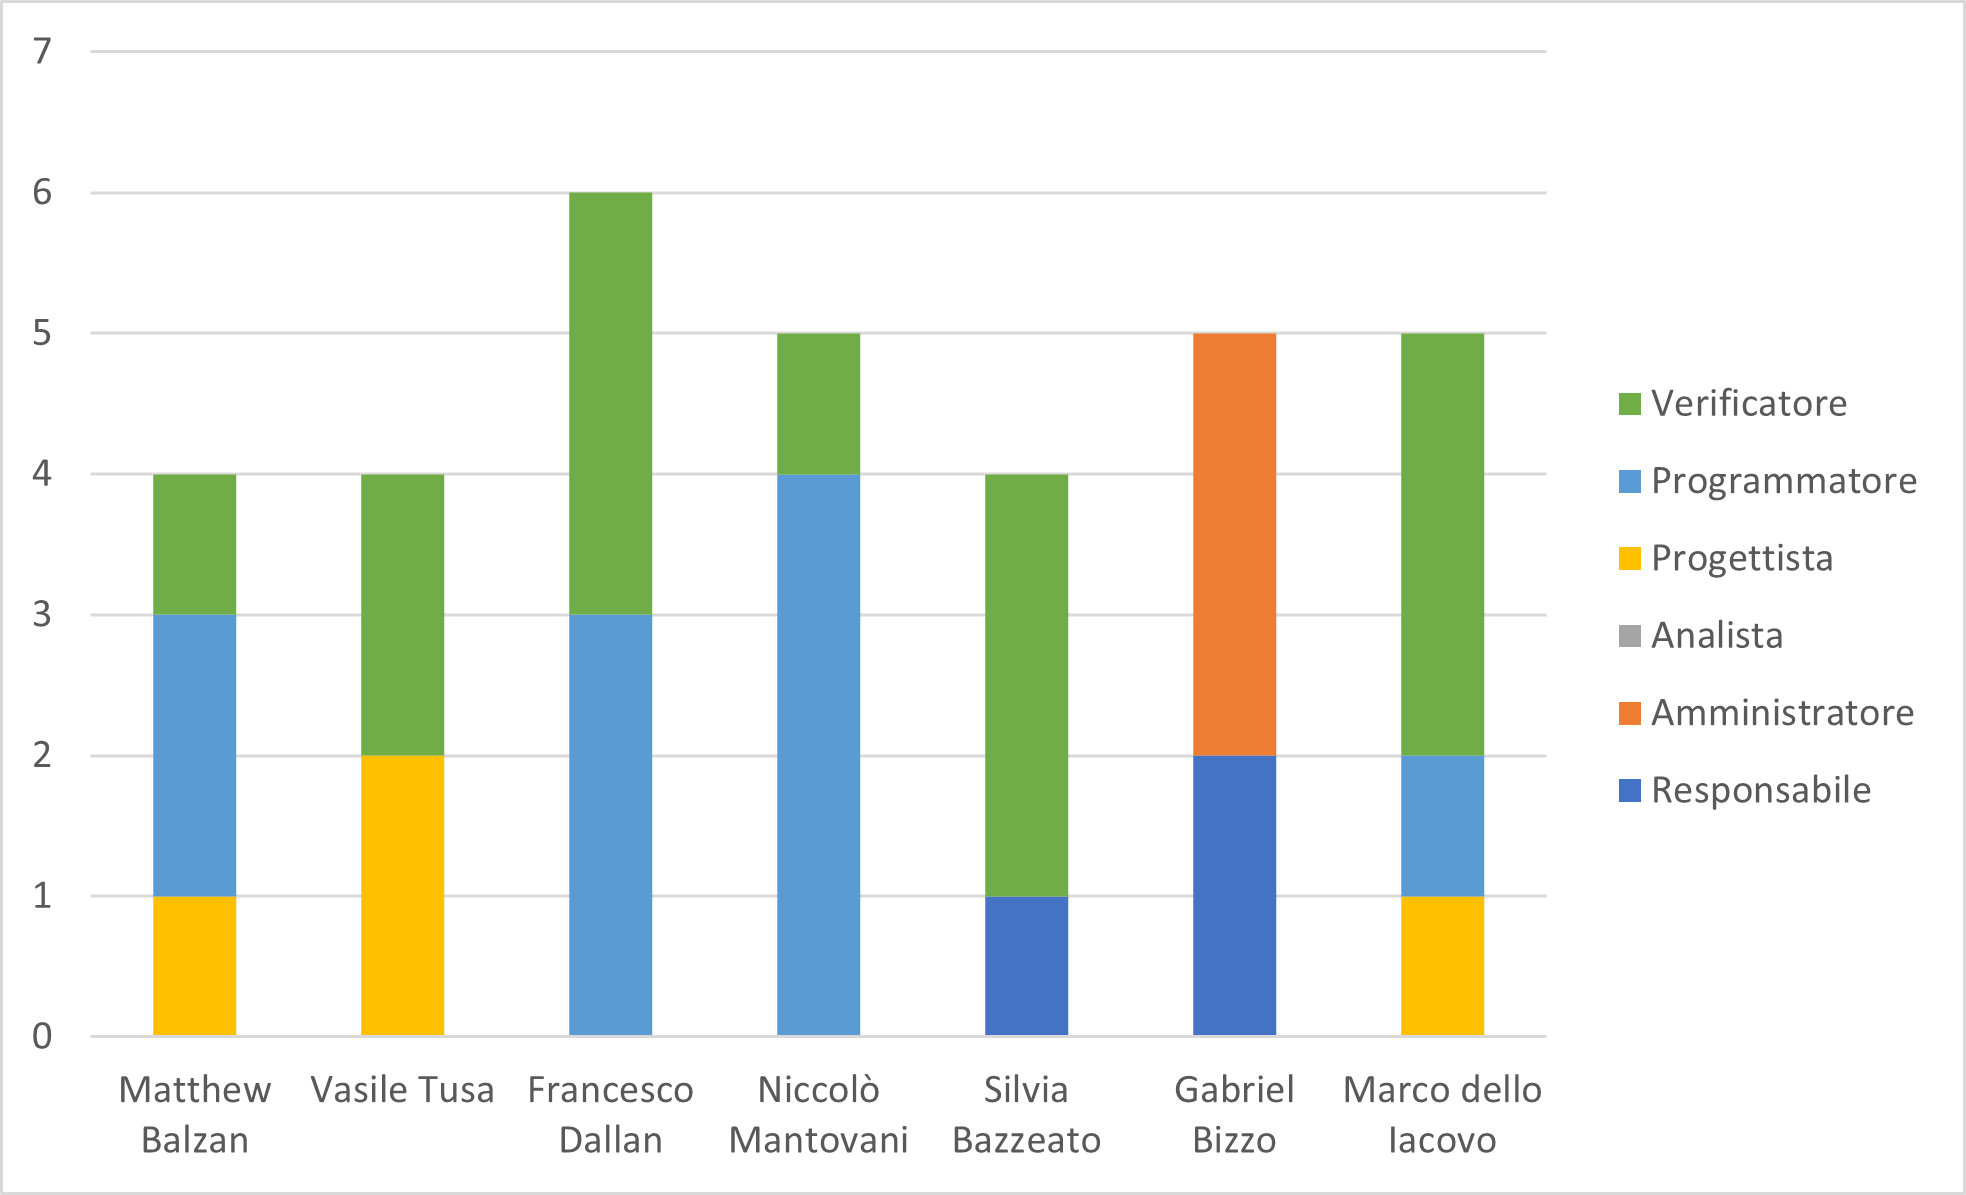
\includegraphics[scale=0.90]{res/Preventivo/Fasi/CodificaIncrementi/istogramma10}\\
\caption{Istogramma della ripartizione dei ruoli nell'incremento 10}
\end{figure}


\myparagraph{Prospetto economico}

In questo incremento, il costo per ogni ruolo è il seguente:

{

\rowcolors{2}{azzurro2}{azzurro3}

\centering
\renewcommand{\arraystretch}{1.8}
\begin{longtable}{C{3cm} C{1cm} C{2cm} }

\rowcolor{azzurro1}
\textbf{Ruolo} &
\textbf{Ore}&
\textbf{Costo}\\
\endhead

\textit{Responsabile} & 3 & 90\euro{} \\
\ammProg & 3 & 60\euro{} \\
\analProg & 0 & 0\euro{} \\
\progetProg & 4 & 88\euro{} \\
\programProg & 10 & 150\euro{} \\
\verifProg & 13 & 195\euro{} \\
\textbf{Totale} & 33 & 583\euro{} \\

\rowcolor{white}
\caption{Prospetto dei costi per ruolo nell'incremento 10}\\

\end{longtable}
}
\newpage
Il seguente areogramma riassume i dati ottenuti:

\begin{figure}[H]
\centering
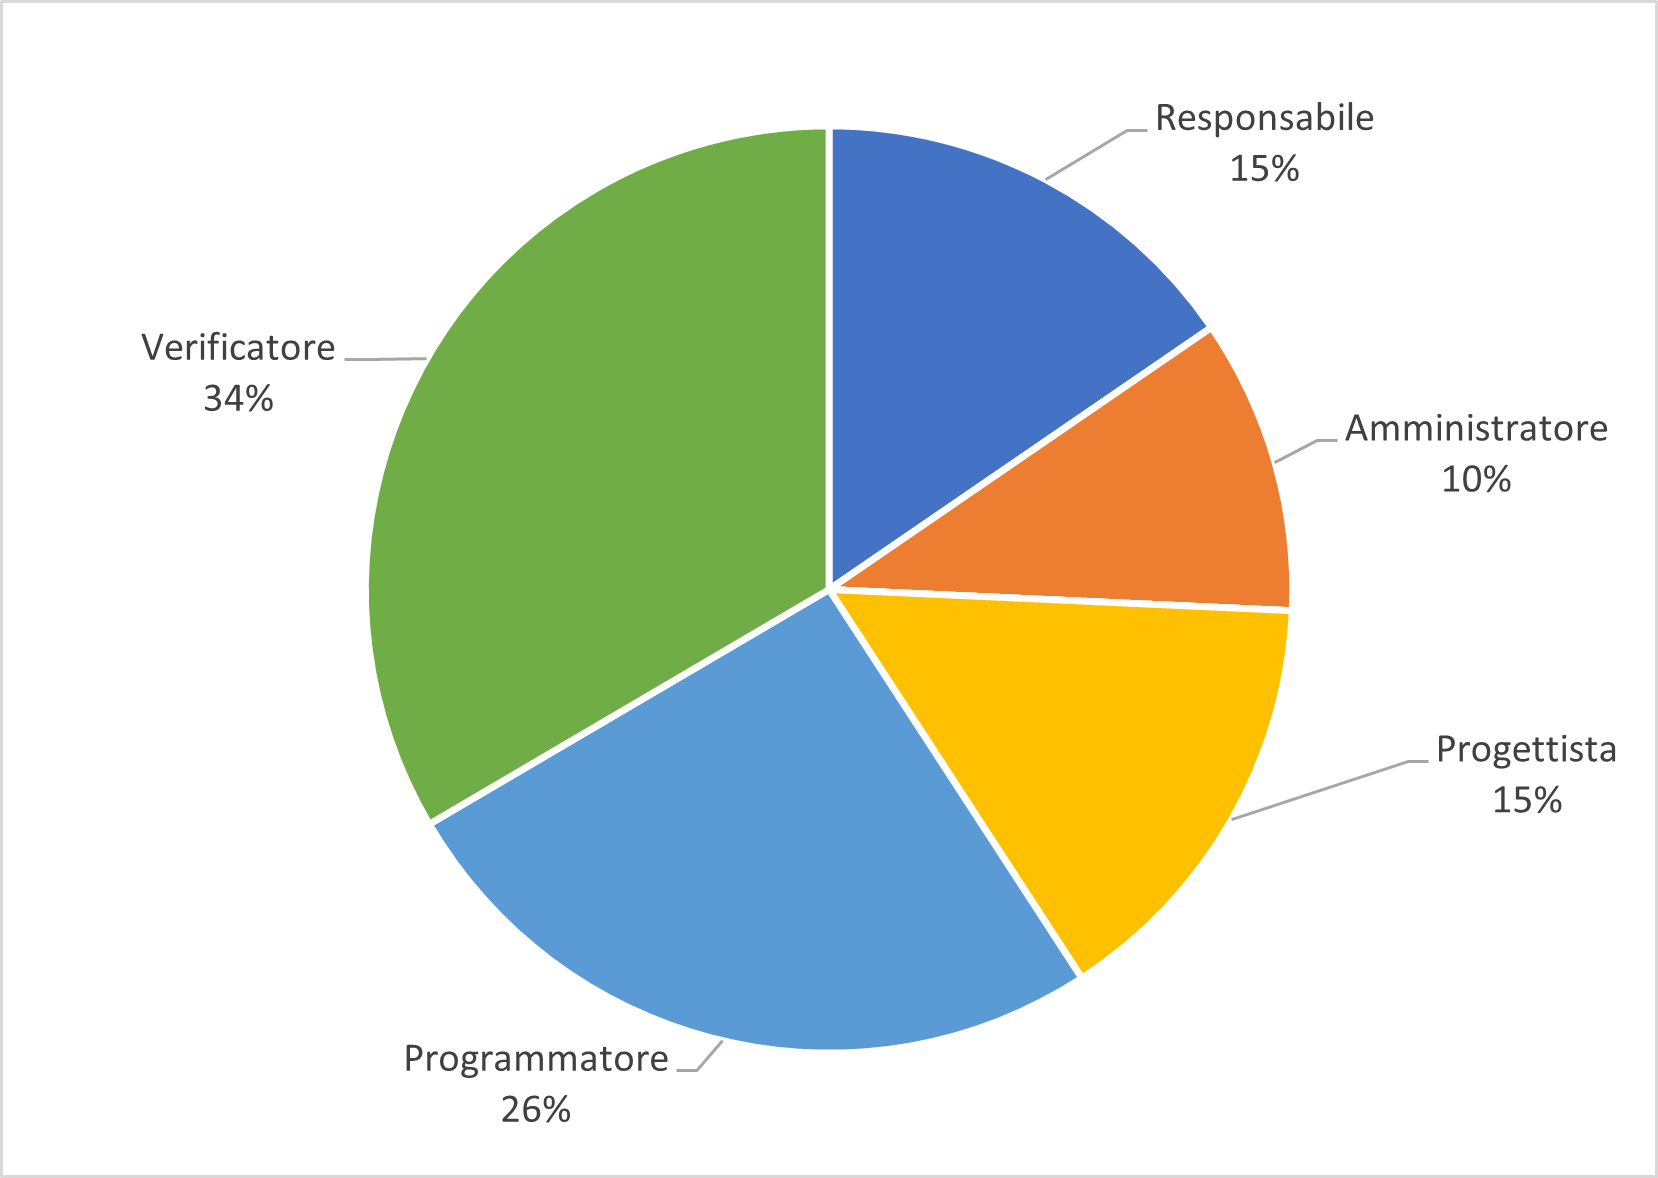
\includegraphics[scale=0.90]{res/Preventivo/Fasi/CodificaIncrementi/torta10}\\
\caption{Areogramma della distribuzione economica nell'incremento 10}
\end{figure}





